\documentclass[12pt,relax]{TrilinosDoc}
% ---------------------------------------------------------------------------- %
%
% Set the title, author, and date
%
\title{An Object-Oriented Model for Parallel Data Redistribution}
\SANDsubtitle{}

\author{Michael A.~Heroux\\
        Numerical and Applied Mathematics Department \\
	   Sandia National Laboratories\\
	   P.O. Box 5800\\
	   Albuquerque, NM 87185-1110 \\
	   maherou@sandia.gov \\
	 }

% There is a "Printed" date on the title page of a SAND report, so
% the generic \date should generally be empty.
\date{}


\SANDnum{SAND2003-xxxx}
\SANDprintDate{February 2003}
\SANDauthor{Michael A.~Heroux, Sandia National Laboratories}


\SANDreleaseType{Unlimited Release}


\SANDdistcategory{UC-999}	% DOE mandates it, but many reports don't have it


% ---------------------------------------------------------------------------- %
%
% Header style
%
\renewcommand{\chaptermark}[1]{\markboth{#1}{}}
\renewcommand{\sectionmark}[1]{\markright{\thesection\ #1}}
\lhead[\fancyplain{}{OO Parallel Data Redistribution}]%
{\fancyplain{}{\rightmark}}
\rhead[\fancyplain{}{\leftmark}]
{\fancyplain{}{OO Parallel Data Redistribution}}
\usepackage{graphicx} 


\begin{document}
\maketitle

\begin{abstract}
This paper presents an object-oriented model for parallel data distribution on
distributed memory parallel computers.
\end{abstract}


\clearpage
\section*{Acknowledgement}
The author would like to acknowledge the support of the ASCI and LDRD programs
that funded development of Trilinos.


\tableofcontents

\section{Introduction}

For our purposes, parallel data redistribution concerns the redistribution of 
data on a parallel distributed memory computer, where all processors on the 
machine are participating in the operation, even though some processor may send
or receive no data..  The data is assumed to be 
partitioned across the machine in some form already, including the case where one
processor owns all of the data.


\section{Basic Parallel Data Redistribution Operations}

An essential design issue in the development of distributed memory parallel programs is the
distribution of data across the memory of the computer.  Optimal distribution of data and work
is an often a multiply-constrained optimization problem with the goal of balancing the work and
data distribution across all nodes of the parallel machine and minimizing the cost of
communicating remote data to processors as needed as the computation proceeds.
Except for embarrassingly parallel programs, access to remote data is required even if
the initial distribution of work and data is optimal.  In the single program multiple data
(SPMD) model, accessing remote data typically involves all processors, even if some processors
are not sending or receiving data.  We use the term {it parallel data
redistribution (PDR)} to refer to the simultaneous exchange of distributed data as it occurs during
the execution of an SPMD program.  The focus of the paper is to develop an object-oriented
model for PDR.  These ideas have been used in the Epetra~\cite{Epetra-Ref-Manual} and
Tpetra~\cite{Tpetra-User-Guide} software packages.

Two of the most common classes of PDR operations are:
\begin{enumerate}
\item Collective operations, such as the dot
product of two distributed vectors, and 
\item Sparse all-to-all operations, where each processor will
communicate with some, but typically not all, other processors.
\end{enumerate}


\subsection{Regular pattern and collective operations}

\subsection{Sparse Matrix Vector Multiplication}

One of the most common pattern-dependent distributed memory kernels is sparse matrix vector multiplication.
This type of kernel appears in many types of applications but is often implemented assuming a
one-dimensional partitioning of the row (or columns) of the matrix such that each row is uniquely and
completely assigned to one processor.  Also, in the square matrix case, the vectors are usually distributed
with a conformal partitioning.  Figure~\ref{MatrixVectorDistribution} illustrates this case for a 4-by-4
problem on two processors.  The first (last) two rows of the matrix and the first (last) two elements of 
both vectors are assigned to PE 0 (PE 1).  Given this distribution, the non-zero pattern of the matrix stored
on each processor determines which elements of $x$ are required to compute $w$.  On PE 0, there are no
non-zero entries in the third column, so that column is not present on PE 0, and the third element of $x$
(stored on PE 1) does not need to be sent to PE 0.  Therefore, locally, the fourth
column of the global matrix become the third column on PE 0, and the fourth global element of $x$ is labeled
as the third elements locally on PE 0, as illustrated in Figure~\ref{PE1MatrixVectorDistribution}.

On PE1, global

\begin{figure} 
\begin{center} 
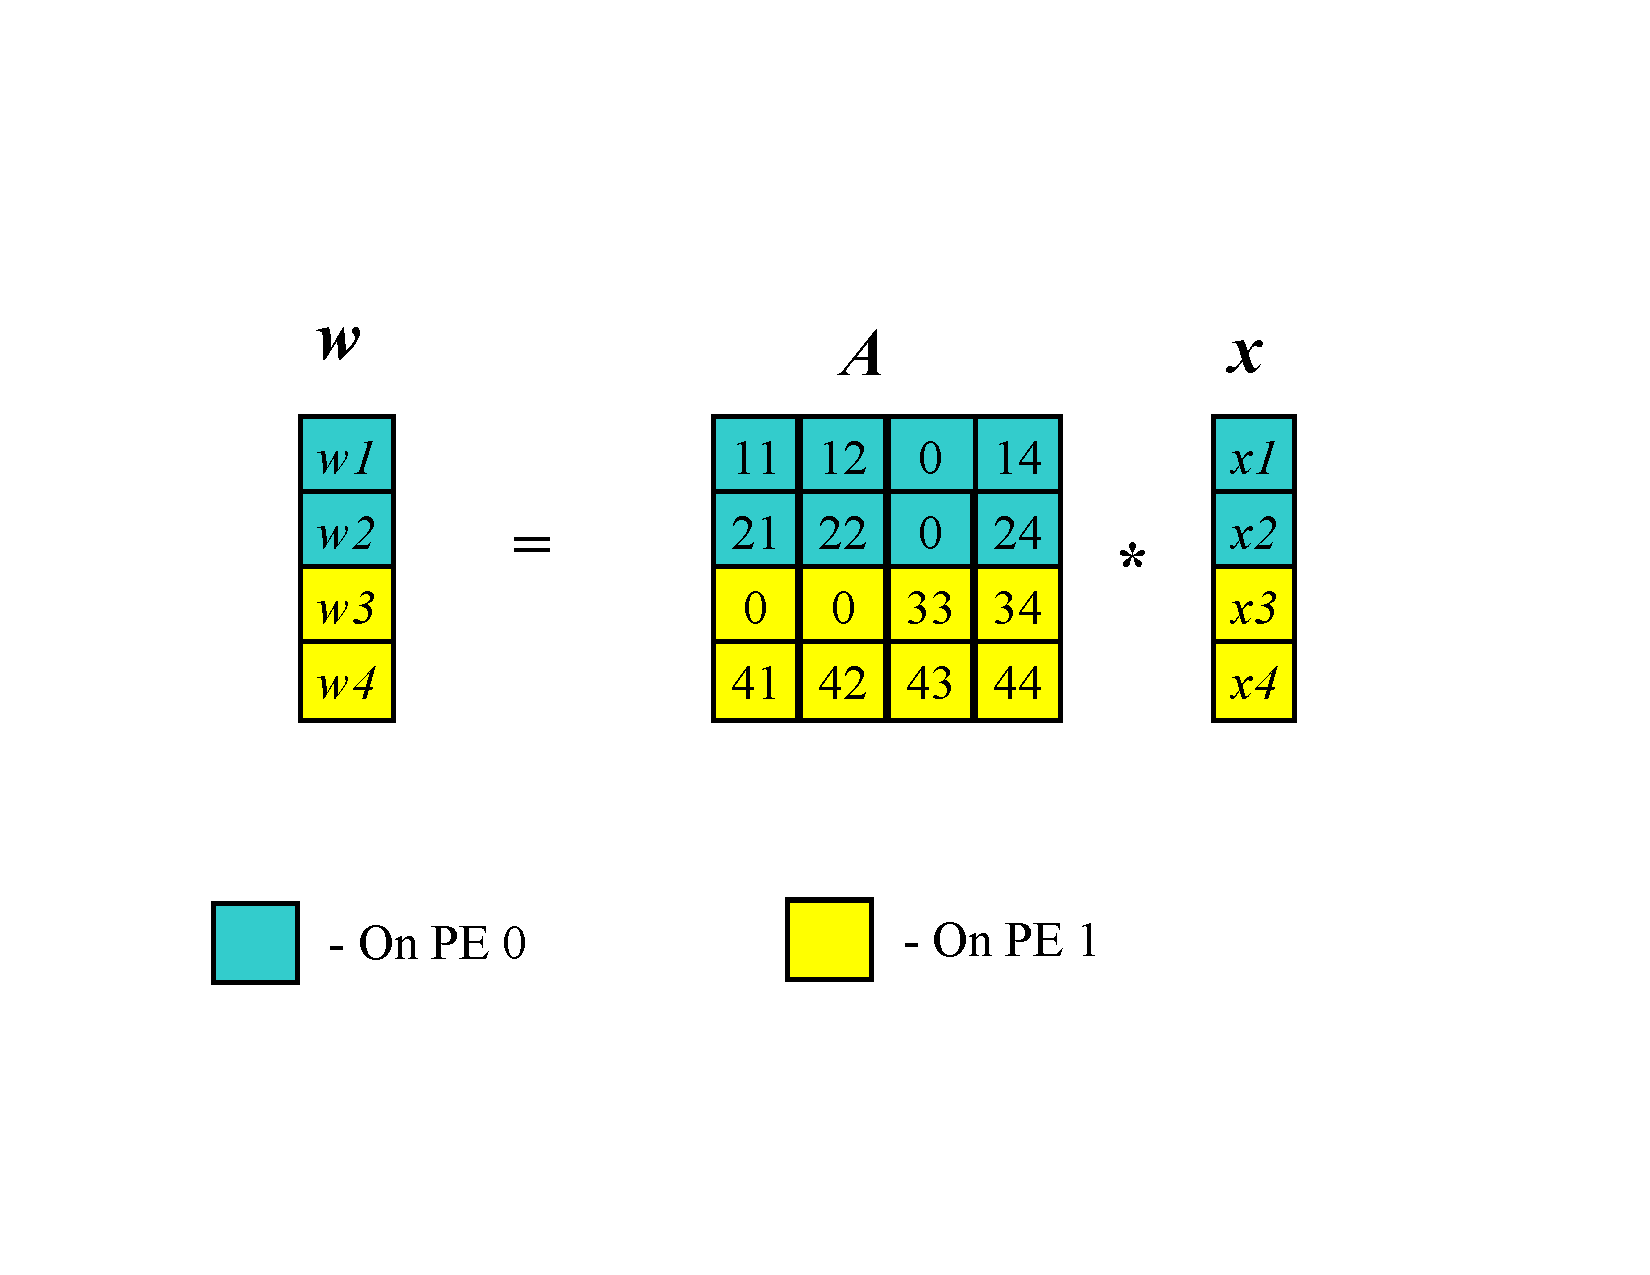
\includegraphics[height=3in]{TwoPESpMV}
\end{center} 
\label{MatrixVectorDistribution}
\caption{Matrix and vector assigments on two memory images}
\end{figure} 

\begin{figure} 
\begin{center} 
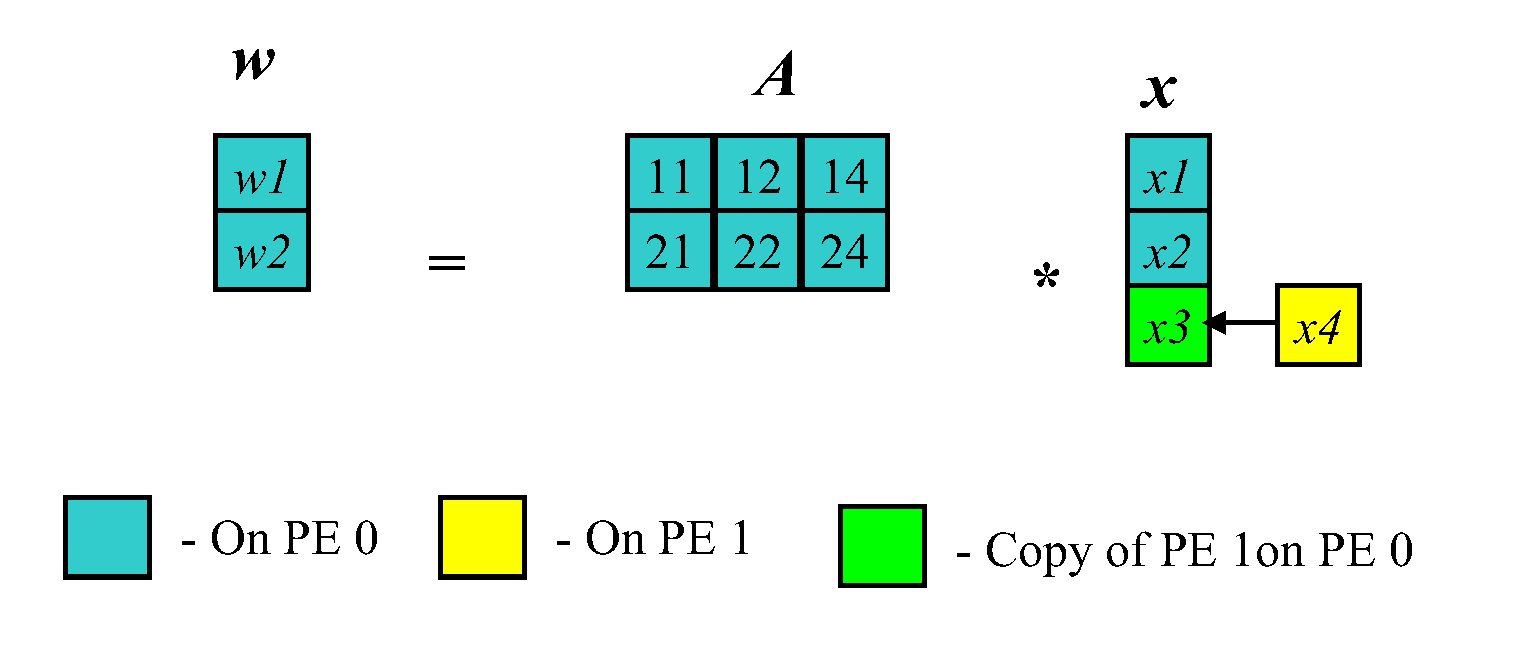
\includegraphics[height=3in]{PE0SpMV}
\end{center} 
\label{PE0MatrixVectorDistribution}
\caption{Contents of memory image on PE 0 after distribution}
\end{figure} 

\begin{figure} 
\begin{center} 
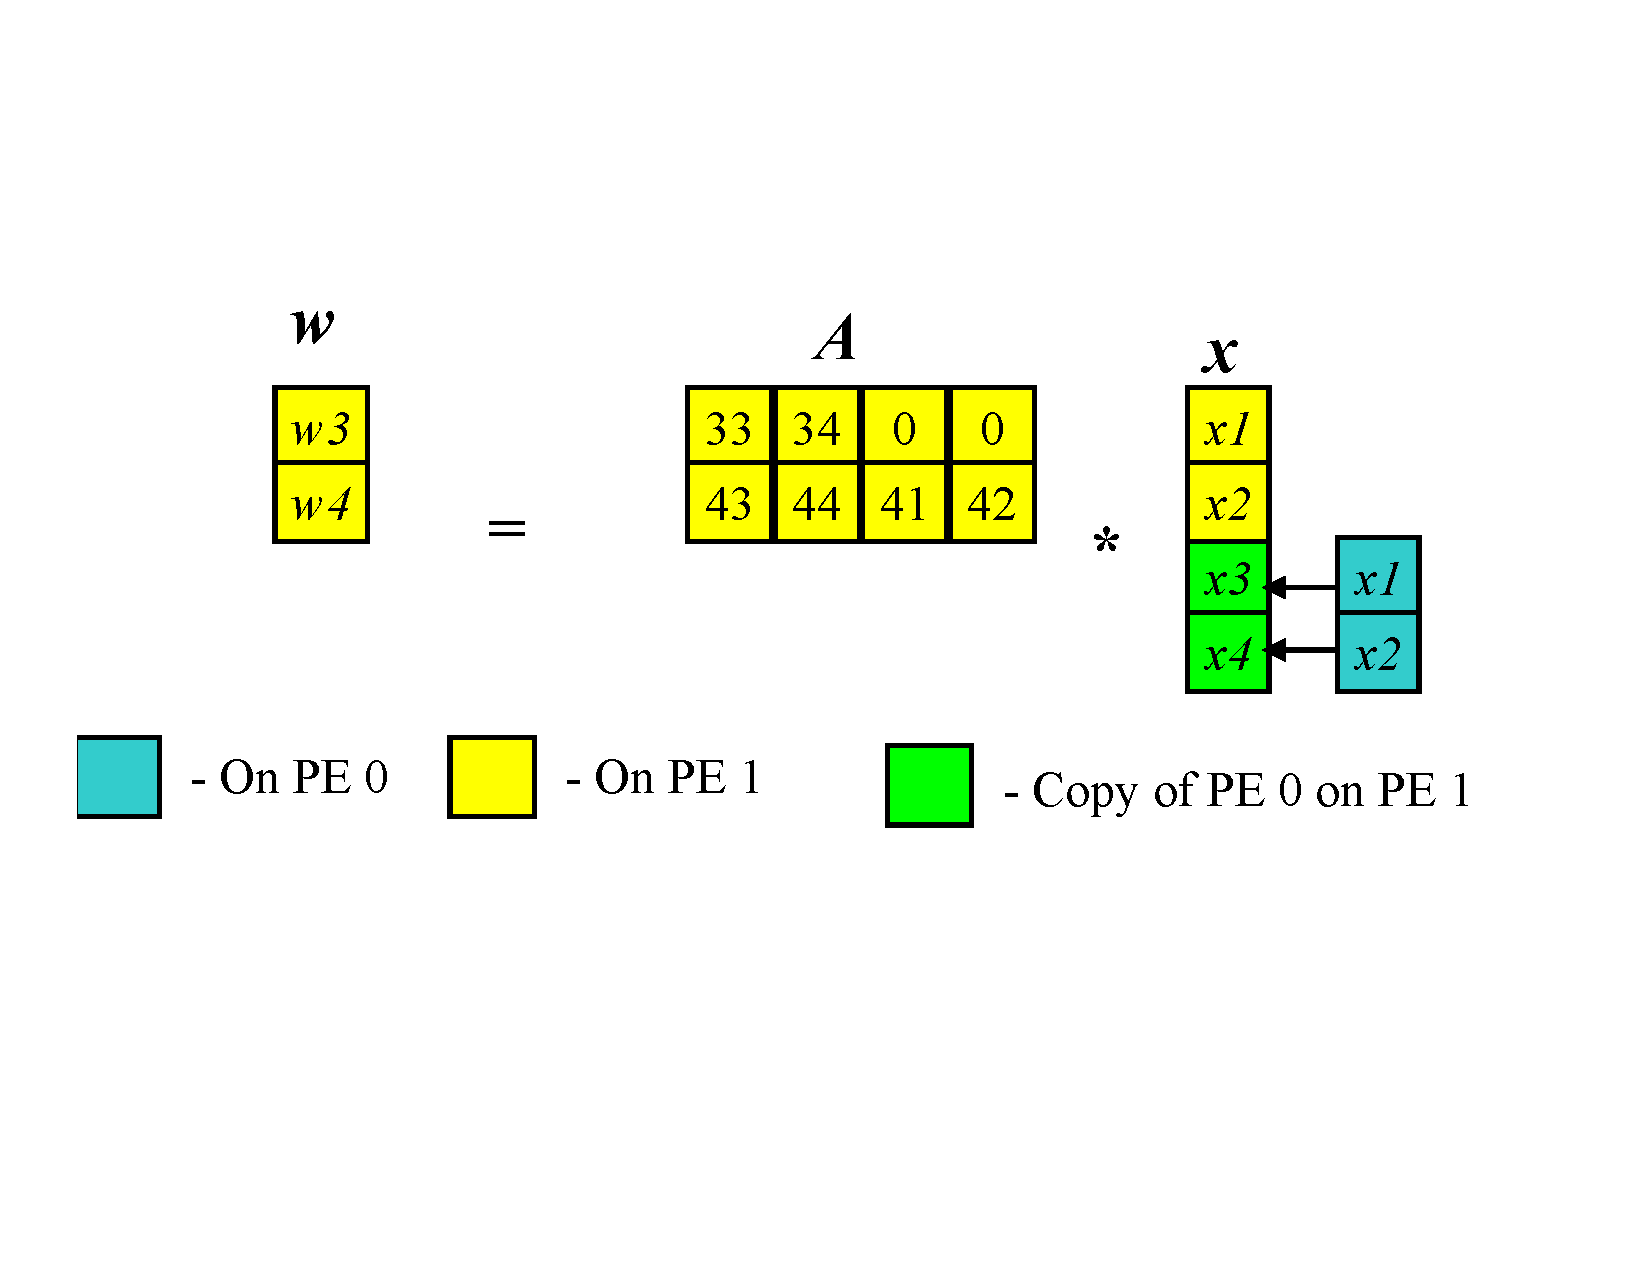
\includegraphics[height=3in]{PE1SpMV}
\end{center} 
\label{PE1MatrixVectorDistribution}
\caption{Contents of memory image on PE 1 after distribution}
\end{figure} 


\section{PDR Terms and Concepts}
\label{sect:concepts}

\subsection{Distributed Objects}

\subsection{Element Spaces and Global IDs}

Given an existing distribution of data, we want a formal mechanism for describing
how the data should be redistributed.  To accomplish this, we define an 
{\it element space} as a collection of labeled elements.  The exact meaning of
an element is determined by the type of object we are redistributing.
The label associated with each element is a signed integer value which we refer to as
the {\it global identifier} or {\it GID} of that element.  If there are no 
repeated GIDs associated with an element space, the element space is said to 
have the one-to-one property.  For many of the redistribution operations, the
one-to-one property is required for one or both of the element spaces involved
in the redistribution operation.

An element space is itself a distributed object.  An Espace is constructed by 
having each processor call the espace constructor, passing in the number of
elements that should be assigned to the processor and a list of related GIDs.

\subsection{Import and Export Operations}

\section{Important PDR Classes}

\subsection{Parallel Machine Class}

\subsection{Element Space Class}

\subsection{Distributed Object Base Class}

\subsection{User Oriented Distributed Object Classes}

\subsection{Import and Export Classes}

\subsubsection{Classification of Global IDs}


\section{Using Imports and Exports for Common PDR Operations}

\subsection{Sparse Matrix Vector Multiplication}

\subsection{Optimal Data Distributions}

\section{Conclusions}


% ---------------------------------------------------------------------- %
% References
%
    \clearpage
    \bibliographystyle{plain}
    \bibliography{OODataRedistribution}
    \addcontentsline{toc}{section}{References}


% ---------------------------------------------------------------------- %
% Appendices should be stand-alone for SAND reports. If there is only
% one appendix, put \setcounter{secnumdepth}{0} after \appendix
%
%    \appendix
%\section{}

% \printindex

    \begin{SANDdistribution}
	\SANDdistExternal{1}{An Address\\ 99 $99^{th}$ street NW\\City, State}
	\SANDdistExternal{3}{Some Address\\ and street\\City, State}
	\bigskip
	\SANDdistExternal{12}{Another Address\\ On a street\\City, State\\U.S.A.}


	\SANDdistInternal{1}{1110}{Rolf Riesen}{9223}

	% Housekeeping copies necessary for every unclassified report:
	\SANDdistInternal{1}{9018}{Central Technical Files}{8940-2}
	\SANDdistInternal{2}{0899}{Technical Library}{4916}
	\SANDdistInternal{2}{0619}{Review \& Approval Desk}{4916}

	% If report has a Patent Caution or Patent Interest, add this:
	\SANDdistInternal{3}{0161}{Patent and Licensing Office}{4916}
    \end{SANDdistribution}

\end{document}
